% Packages utilisés :
%
% \usepackage[french]{babel}
% \usepackage[utf8x]{inputenc}
% \usepackage{amsmath}
% \usepackage{amssymb}
% \usepackage{tikz}
% \usepackage{tkz-graph}
% \usepackage{algorithm}
% \usepackage{algorithmic}
%
% Il y a aussi besoin d'un environnement solution
% Les questions 3 et 4 ont été réalisées avec l'aide 
% de Guillaume Derval

\section{Séance 3}


\paragraph{1. } Lorsque toutes les arêtes d'un graphe sont de longueur 1, la recherche en largeur dans le graphe permet de trouver le plus court chemin du nœud $s$ au nœud $t$. Quelle est la complexité de cet algorithme? Quel est le pire cas?

\begin{solution}
  Étant donné que cet algorithme doit, au plus, parcourir toutes les arêtes pour trouver le chemin,
  on a une complexité en $\bigoh(\vert E \vert)$, avec $\vert E \vert$ le nombre d'arêtes dans le graphe.

  Le pire des cas (celui où le nombre d'arêtes est le plus élevé) est le cas du graphe complet.
  En effet, par le théorème des poignées de mains, on a que $\vert E \vert = \frac{n(n-1)}{2}$.
  La complexité est donc $\bigoh(n^2)$, avec $n$ le nombre de nœuds dans le graphe.
\end{solution}

\paragraph{2. } Lorsque certaines longueurs dans un digraphe sont négatives il peut être nécessaire de devoir faire la distinction entre la plus courte chaîne et le plus court chemin. Donnez l'exemple d'un graphe pour lequel cette distinction est nécessaire. Cette distinction est-elle nécessaire si tous les circuits sont de longueur positive?
\begin{solution}
Une chaîne \footnote{même chose qu'un parcours} est une suite $v_0e_1v_1e_2...e_nv_n $ où $v_1,v_2,...$ sont des sommets et $e_1,e_2,...$ sont des arêtes.  Un chemin est une chaîne dont les sommets sont tous distincts.

Un digraphe est graphe dirigé, ce qui est important ici car si le graphe n'était pas dirigé et qu'un poids
était négatif, il suffirait de faire cette arête en aller-retour suffisamment de fois pour avoir un poids aussi petit que l'on veut.
Pour un digraphe, ce n'est pas aussi simple, le fait qu'il y ait des arêtes de longueur négative ne signifie pas spécialement que la plus courte chaîne sera différente que le plus court chemin.

  Dans le graphe suivant, si on veut trouver le chemin de poids minimum de $A$ à $E$, on a $ABDE$ de poids $8$.
  Par contre, il n'y a pas de plus courte chaîne car $w(AB(DCBD)^nE) = 8 - 18n$ peut être aussi
  petit que l'on veut.

  \begin{center}
    \begin{tikzpicture}[transform shape]
      \SetGraphUnit{2}
      \Vertex[L=$A$]{A}
      \EA[L=$B$](A){B}
      \SOEA[L=$C$](B){C}
      \NOEA[L=$D$](B){D}
      \SOEA[L=$E$](D){E}
      \SetUpEdge[style={->},
      labelstyle = {draw}]
      \Edge[label=$20$](A)(B)
      \Edge[label=$-5$](B)(D)
      \Edge[label=$-15$](D)(C)
      \Edge[label=$2$](C)(B)
      \Edge[label=$3$](D)(E)
    \end{tikzpicture}
  \end{center}

  Cependant, cette distinction n'est seulement nécessaire lorsqu'il y a
  un circuit de longueur négative comme ici avec $DCBD$.
  Démontrons le par l'absurde.\\

  Supposons que la plus courte chaîne et le plus court chemin sont différents. Il y a deux possibilités :
  \begin{itemize}
    \item Soit le plus court chemin est plus court ou égal à la plus courte chaîne. Dans ce cas, il existe une plus courte chaîne que celle trouvée précédemment, c'est à dire le plus court chemin.
    \item Soit la plus courte chaîne est plus courte que le plus court chemin.
      Nous savons que pour qu'une chaîne soit la plus courte entre $u$ et $v$,
      il faut qu'elle soit aussi la plus courte entre deux nœuds intermédiaires du graphe,
      supposons que le cycle comprenne deux fois le nœud $w$,
      pour que la chaîne soit optimale, il faut que le chemin entre w et w soit optimal,
      or le cycle a une longueur strictement positive,
      on peut donc trouver un chemin plus court entre $w$ et $w$ de taille 0 (ne pas faire le cycle).
      La chaîne trouvée précédemment n'est donc pas optimale, on obtient donc une contradiction,
      on utilise le même argument pour tout les cycles du graphes.
  \end{itemize}
\end{solution}

\paragraph{3. } L'algorithme de Dijkstra ne fonctionne correctement que lorsque la longueur des arêtes est positive. Donnez un exemple d'un digraphe dont tous les cycles sont de longueur positive et pour lequel l'algorithme de Dijkstra ne fournit pas la bonne solution. (A faire chez vous) Proposez une modification de l'algorithme de Dijkstra pour qu'il donne la bonne solution, même dans le cas où certaines arêtes sont négatives, si tous les cycles sont de longueur positive.

\begin{solution}
  Nous allons tout d'abord appliquer l'algorithme de Dijkstra sur le graphe suivant pour trouver le chemin de poids minimum entre A et B.
        \begin{center}		
			\begin{tikzpicture}[scale=0.75,transform shape]
  				\Vertex[x=0,y=0]{A}
  				\Vertex[x=3,y=0]{B}
  				\Vertex[x=0,y=-3]{C}
  				\tikzset{LabelStyle/.style =   {draw}}
  				\tikzstyle{EdgeStyle}=[post]
  				\Edge[label=$1$](A)(B)
  				\Edge[label=$5$](A)(C)
  				\Edge[label=$-10$](C)(B)
			\end{tikzpicture}
		\end{center}
		Ce digraphe, qui ne possède pas de cycle, ne gère pas bien Dijkstra. En effet, l'algorithme va parcourir l'arête de poids $1$ et ignorer l'arête de poids $5$ car cette dernière est plus lourde et on trouve directement la destination en parcourant celle de poids $1$. En résumé, l'algorithme nous renvoie un chemin de longueur $1$ alors que le chemin de plus petit poids est de poids $-5$.\\
		
		Proposons maintenant des alternatives à l'algorithme de Dijkstra. La méthode "simple" est de remettre à jour les nœuds précédents si l'on repasse par une arête de poids négatif. En revanche, cette technique est exponentielle en complexité. Une alternative plus intéressante est l'algorithme de Bellman-Ford, qui fonctionne sur les graphes sans cycle de poids négatif et est de complexité $\bigoh(nm)$, avec $n$ le nombre de nœuds dans le graphe et $m$ le nombre d'arêtes.\\
		
		Un exemple de pseudo-code pour l'algorithme de Bellman-Ford :
		\begin{algorithm}{Bellman-Ford(List $vertices$, List $edges$, Vertex $source$)}
			\begin{algorithmic}
				\REQUIRE Un graphe (ici, représenté sous forme d'une liste de nœuds et une liste d'arêtes) et un nœud source
				\ENSURE Un tableau contenant les distances de nœuds par rapport au nœud de départ et un tableau contenant des références vers le prédécesseur de chaque nœud. S'il y a un cycle négatif, une valeur qui l'indique est renvoyée.
				
				\medskip
				\STATE \textit{//Initialisation}
				\FORALL{$v$ in $vertices$}
					\IF{$v\ ==\ source$}
						\STATE $distance[v] \leftarrow 0$
					\ELSE
						\STATE $distance[v] \leftarrow +\infty$
					\ENDIF
					\STATE $predecessor[v] \leftarrow\ null$	
				\ENDFOR
				
				\medskip
				\STATE \textit{//Mise à jour des distances et des prédécesseurs}		
				\FORALL{$u$ in $vertices$}
					\FORALL{$edge(u,v)$ with weight $w$ in $edges$}
						\IF{$distance[v] > distance[u] + w$}
							\STATE $distance[v] \leftarrow distance[u] + w$
							\STATE $predecessor[v] \leftarrow u$
						\ENDIF
					\ENDFOR			
				\ENDFOR
				
				\medskip
				\STATE \textit{//Vérification pour les cycles de poids négatif}
				\FORALL{$edge(u,v)$ with weight $w$ in $edges$}
					\IF{$distance[v] > distance[u] + w$}
						\STATE \textbf{return} "il y a un cycle négatif"
					\ENDIF
				\ENDFOR
				\medskip
				
				\STATE \textbf{return} les tableaux "predecessor" et "distance"
			\end{algorithmic}
		\end{algorithm}	
		
		Dans le cas de notre exemple, l'algorithme procède comme suit :
		\begin{enumerate}
			\item Initialisation : distance[A] :$= 0$, distance[B] :$= +\infty$, distance[A] :$= +\infty$
			\item On trouve B, on met sa distance à $1$ et son prédécesseur à A
			\item On trouve C, on met sa distance à $5$ et son prédécesseur à A
			\item On trouve B, comme on a que $1>5+(-10)$, on met sa distance à $-5$ et son prédécesseur à $C$
			\item Il n'y a pas de cycle de poids négatif.
			\item Le poids du plus petit chemin entre A et B est la distance de B. Pour trouver les nœuds intermédiaires du chemin, il suffit de regarder les prédécesseurs.
		\end{enumerate}
\end{solution}

\paragraph{4. } Soit $d_k(j)$ la longueur du plus court chemin de $s$ à $j$ avec au plus $k$ arêtes. Trouvez une récurrence pour $d_k(j)$. Démontrez que $d_{n-1}(j)$ est la plus courte distance de $s$ à $j$.

\begin{solution}
On écrit que la longueur du plus court chemin de $s$ à $j$ avec au plus $k$ arêtes est égal au minimum entre le plus court chemin de $s$ à $j$ de longueur $k-1$ et le chemin minimum de $s$ à $i$ de longueur $k-1$ + l'arête de $i$ à $j$.
$$d_k(j) = min (d_{k-1}(j) , min_i(d_{k-1}(i)+w(i, j))$$
La récurrence ainsi établie nous permet de démontrer que $d_{n-1}(j)$ est la distance minimale entre $s$ et $j$. Il est évident que $d_k(j)\ge d_{n-1}(j)\ \forall k \le n-1$ (par la simple définition de la récurrence qui prend toujours le minimum du pas précédent). De plus, $d_k(j) = d_{n-1}(j)\ \forall k \ge n-1$ car le fait de prendre une $n$ième arète supplémentaire provoque l'apparition d'un cycle(par les propriétés des arbres). L'apparition de ce cycle provoque un allongement superflu du chemin, d'où $min_i(d_{k-1}(i)+w(i, j)) \ge d_{k-1}(j)$ et donc $d_k = d_{k-1}\ \forall k \ge n-1$.
\end{solution}

\paragraph{5. } Le graphe dirigé ci-dessous est acyclique. Utilisez l'algorithme de Dijkstra pour trouver le plus court chemin du noeud $1$ à chaque autre noeud du graphe.

\begin{center}
  \begin{tikzpicture}[x=2cm,y=1cm]
    \Vertex{1}
    \NOEA(1){2}
    \SOEA(1){3}
    \SOWE(3){4}
    \SOEA(4){7}
    \NOEA(3){5}
    \SOEA(3){6}

    \SetUpEdge[style={->}]
    \Edge[label=$12$](1)(2)
    \Edge[label=$4$](1)(4)
    \Edge[label=$5$](2)(5)
    \Edge[label=$4$](3)(2)
    \Edge[label=$7$](3)(5)
    \Edge[label=$3$](3)(7)
    \Edge[label=$3$](4)(3)
    \Edge[label=$4$](4)(7)
    \Edge[label=$3$](5)(6)
    \Edge[label=$9$](7)(6)
  \end{tikzpicture}
\end{center}

\begin{solution}
  La matrice associée à l'algorithme de Dijkstra est donnée par :
  \[
    \mathcal{D}=
    \begin{pmatrix}
      1 & 2   & 3       & 4  & 5          & 6 & 7 \\
      \boxed{0} & 12 & \infty & 4 & \infty    &\infty & \infty  \\
      \boxed{0} & 12 & 7       & \boxed{4} & \infty    & \infty  & 8  \\
      \boxed{0} & 11 & \boxed{7}       &\boxed{4} & 14         & \infty  & 8\\
      \boxed{0} & 11 & \boxed{7}       & \boxed{4}& 14         & 17 & \boxed{8}\\
      \boxed{0} & \boxed{11} & \boxed{7}       & \boxed{4} & 14         & 17 &  \boxed{8}\\
      \boxed{0} & \boxed{11} & \boxed{7}      & \boxed{4} & \boxed{14}         & 17 &  \boxed{8}\\
      \boxed{0} & \boxed{11}& \boxed{7}       & \boxed{4} & \boxed{14}         & \boxed{17} &  \boxed{8}\\
    \end{pmatrix}.
  \]
\end{solution}

\paragraph{6. } Vous avez deux seaux d'une contenance de 7 et 5 litres. Vous avez besoin de 4 litres. Les opérations permises sont les suivantes : remplir un seau, vider un seau, verser le contenu d'un seau dans l'autre jusqu'à ce que le seau soit rempli ou l'autre vide. Vous souhaitez effectuer un nombre minimum d'opérations et obtenir un seau contenant 4 litres. Formulez ce problème comme un problème de plus court chemin, et trouvez-en la solution.

\begin{solution}
Le problème peut être modélisé comme le plus court chemin entre le nœud (0,0) et (0,4) dans le graphe donné. Il suffit de suivre la chaîne, on obtient sept opérations nécessaires. Nous n'avons tracé que les arêtes permettant d'aller dans les deux sens, par exemple, nous n'avons pas tracer  l'arête entre (5;4) et (5;0) car on peut aller de (5;4) à (5;0) mais pas de (5;0) à (5;4). On peut constater que le chemin le plus court est de 7 opérations. Il est tracé en rouge.
\begin{center}
\begin{tikzpicture}[scale=0.75,transform shape]
  \Vertex[x=-10,y=0]{0;0}
  \Vertex[x=-8,y=2]{0;7}
  \Vertex[x=-8,y=-2]{5;0}
  \Vertex[x=-6,y=2]{5;2}
  \Vertex[x=-6,y=-2]{0;5}
  \Vertex[x=-4,y=2]{0;2}
  \Vertex[x=-4,y=-2]{5;5}
  \Vertex[x=-2,y=2]{2;0}
  \Vertex[x=-2,y=-2]{3;7}
  \Vertex[x=0,y=2]{2;7}
  \Vertex[x=0,y=-2]{3;0}
  \Vertex[x=2,y=2]{5;4}
  \Vertex[x=2,y=-2]{0;3}
  \Vertex[x=4,y=2]{0;4}
  \Vertex[x=4,y=-2]{5;3}
  \Vertex[x=6,y=2]{4;0}
  \Vertex[x=6,y=-2]{1;7}
  \Vertex[x=8,y=2]{4;7}
  \Vertex[x=8,y=-2]{1;0}
  \Vertex[x=10,y=2]{5;6}
  \Vertex[x=10,y=-2]{0;1}
   \Vertex[x=12,y=2]{0;6}
  \Vertex[x=12,y=-2]{5;1}
  \tikzset{LabelStyle/.style =   {draw}}
  %\tikzstyle{LabelStyle}=[fill=white,sloped]
  \tikzstyle{EdgeStyle}=[double = red]
  \Edge(4;0)(0;4)
  \Edge(0;4)(5;4)
  \Edge(5;4)(2;7)
 \Edge(2;7)(2;0)
  \Edge(2;0)(0;2)
  \Edge(0;2)(5;2)
 \Edge(5;2)(0;7)
  \Edge(0;7)(0;0)
  \tikzstyle{EdgeStyle}=[]
    \Edge(0;0)(5;0)
  \Edge(5;0)(0;5)
  \Edge(0;5)(5;5)
 \Edge(5;5)(3;7)
  \Edge(3;7)(3;0)
  \Edge(3;0)(0;3)
  \Edge(0;3)(5;3)
  \Edge(5;3)(1;7)
 \Edge(1;7)(1;0)
  \Edge(1;0)(0;1)
  \Edge(0;1)(5;1)
  \Edge(5;1)(0;6)
  \Edge(0;6)(5;6)
 \Edge(5;6)(4;7)
  \Edge(4;7)(4;0)
\end{tikzpicture}
\end{center}
\end{solution}

\paragraph{7. }
	Vous possédez un billet de $p$ euros et vous souhaitez le changer en pièces de $a_1, a_2, ..., a_k$ euros (tous les montants étant entiers). Est-ce possible? Si oui, avec quel nombre de pièces? Formulez ce problème comme un problème de plus court chemin dans un graphe.


\begin{solution}
	Créons un digraphe de la manière suivante : $p+1$ nœuds numéroté de $0$ à $p$ et des arêtes telles qu'une arête associée à une pièce de valeur $a_k$ relie un nœud $i$ à un nœud $i+a_k$\footnote{à condition de ces deux nœuds à relier soient bien compris entre $0$ et $p$}. Il suffit ensuite d'appliquer l'algorithme de Dijkstra au graphe créé pour chercher le plus petit chemin entre les nœuds $0$ et $p$. Si l'algorithme ne trouve pas de chemin, il est alors impossible d'échanger le montant $p$ avec les pièces disponibles. Vous pouvez regarder quelques exemples ci-dessous.\\
\begin{center}
	\begin{tikzpicture}[scale=0.75,transform shape]
		\Vertex[x=-10,y=0]{0}
 		\Vertex[x=-8,y=0]{1}
		\Vertex[x=-6,y=0]{2}
		\Vertex[x=-4,y=0]{3}
		\tikzset{LabelStyle/.style =   {draw}}
	 	\tikzstyle{EdgeStyle}=[bend left]
	 	\Edge(0)(2)
	 	\tikzstyle{EdgeStyle}=[bend right]
		\Edge(1)(3)
 	\end{tikzpicture}
\end{center}

	Premièrement, un exemple où il n'existe pas de parcours du nœud $0$ au nœud $p$ avec $p=3$ et $a_1 = 2$. En effet, il n'est pas possible d'échanger $3$ euros avec des pièces de $2$ euros.\\

	Deuxièmement, un exemple ou il existe un parcours de $0$ à $p$ avec $p=5$, $a_1=2$ et $a_2=1$. Le chemin le plus court est tracé en rouge et correspond à $2$ pièces de $2$ et une pièce de $1$. Il existe deux autres chemins de même longueur (donc équivalents).\\

\begin{center}
	\begin{tikzpicture}[scale=0.75,transform shape]
		\Vertex[x=-10,y=0]{0}
		\Vertex[x=-8,y=0]{1}
		\Vertex[x=-6,y=0]{2}
		\Vertex[x=-4,y=0]{3}
		\Vertex[x=-2,y=0]{4}
		\Vertex[x=0,y=0]{5}
		\tikzset{LabelStyle/.style =   {draw}}
		\tikzstyle{EdgeStyle}=[bend left,double=red]
		\Edge(0)(1)
		\tikzstyle{EdgeStyle}=[bend left]
		\Edge(1)(2)
		\Edge(2)(3)
		\Edge(3)(4)
		\Edge(4)(5)
		\tikzstyle{EdgeStyle}=[bend right, double = red]
		\Edge(1)(3)
		\Edge(3)(5)
		\tikzstyle{EdgeStyle}=[bend right]
		\Edge(0)(2)
	  	\Edge(2)(4)
 	\end{tikzpicture}
\end{center}

\end{solution}
